\documentclass[../piano_di_progetto.tex]{subfiles}

\begin{document}

La pianificazione si è basata sulle scadenze descritte in \ref{sub:scad}; il gruppo ha scelto di suddividere il periodo che va dalla formazione alla Revisione di Accettazione nelle seguenti fasi:
\begin{itemize}
\item Analisi dei requisiti;
\item Progettazione architetturale;
\item Progettazione di dettaglio e codifica;
\item Validazione e collaudo
\end{itemize}
Ad ognuna di queste attività verranno destinate delle risorse di seguito descritte.


\subsection{Analisi}%
\label{sub:analisi}
Questa attività si svolge nel periodo che va dalla formazione del gruppo alla consegna della \glossario{Revisione dei Requisiti}. In questo periodo il gruppo inizia con la visione dei \glossario{capitolati} proposti, e per ognuno di essi traccia un prototipo di \glossario{studio di fattibilità} dove vengono evidenziati gli aspetti positivi e negativi di ciascuno. Nel frattempo vengono stabilite delle \glossario{norme di progetto}, utili a fissare degli standard di utilizzo ai quali il gruppo si deve attenere. Successivamente alla scelta del capitolato vengono tracciati i requisiti minimi richiesti dal proponente, inoltre il gruppo incontra l’azienda tramite meeting online allo scopo di risolvere eventuali dubbi. 

\begin{figure}[H]
\centering
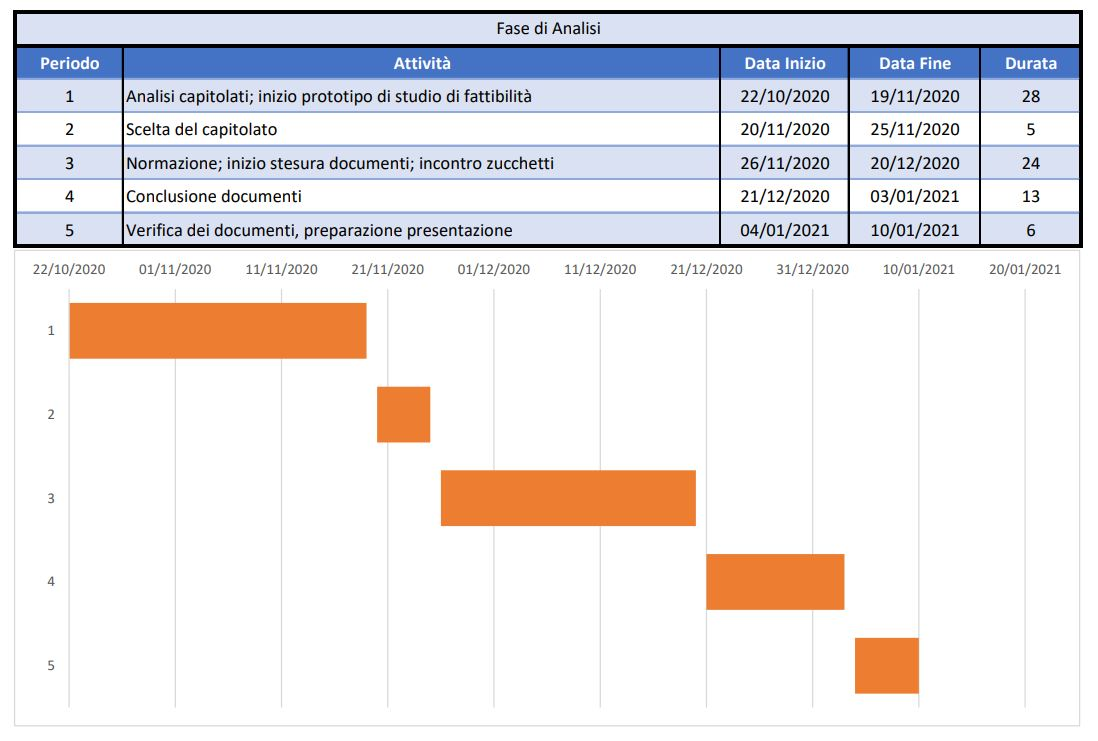
\includegraphics[width=12cm]{fase_analisi}
\caption{ \glossario{Diagramma di Gantt} della fase di analisi dei requisiti}
\end{figure}


\subsection{Progettazione architetturale}%
\label{sub:prog_arc}
La fase di progettazione architetturale inizia subito dopo la consegna della Revisione dei Requisiti, e prevede l’approfondimento delle tecnologie richieste attraverso lo studio autonomo. \\
In questo periodo vi sarà un eventuale aggiornamento delle norme di progetto e sarà aggiornata la pianificazione. Inoltre verrà fatto uno studio più approfondito delle tecnologie coinvolte nel progetto, al fine di realizzare un \glossario{Proof of Concept} che farà da base per la fase successiva.

\begin{figure}[H]
\centering
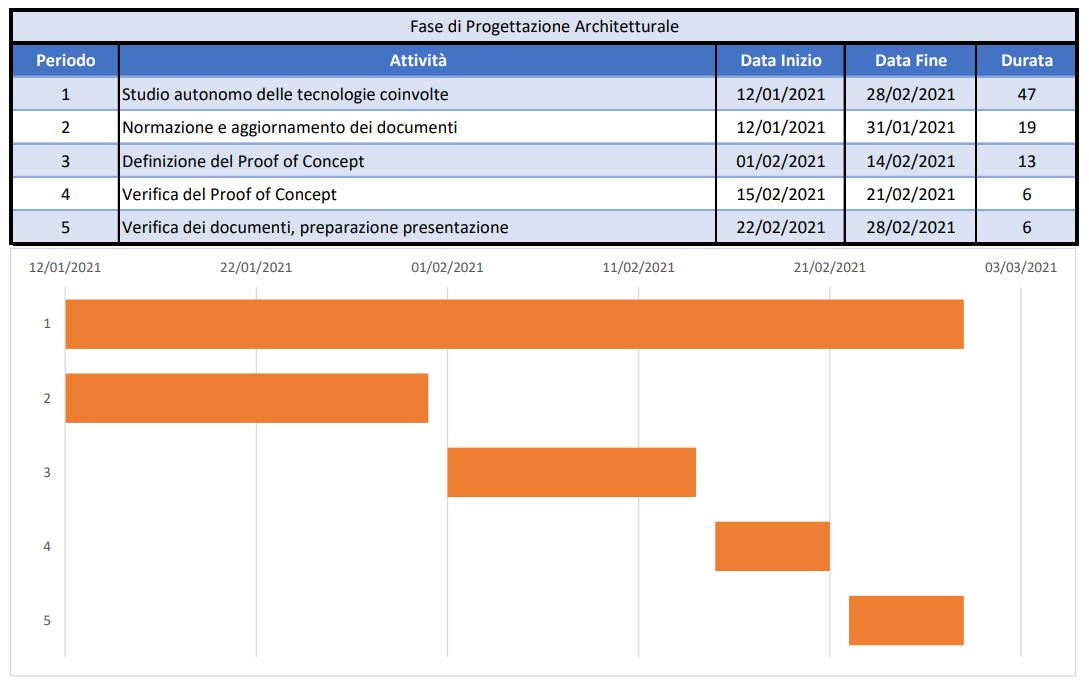
\includegraphics[width=12cm]{fase_prog_archit}
\caption{Diagramma di Gantt della fase di progettazione architetturale}
\end{figure}


\subsection{Progettazione di dettaglio e codifica}%
\label{sub:prog_dett}
Questa fase prevede la stesura del codice sulla base dei dettagli precedentemente tracciati; vi saranno aggiustamenti della pianificazione e aggiornamenti dei documenti. Verrà inoltre redatto il \glossario{manuale d’utente}.

\begin{figure}[H]
\centering
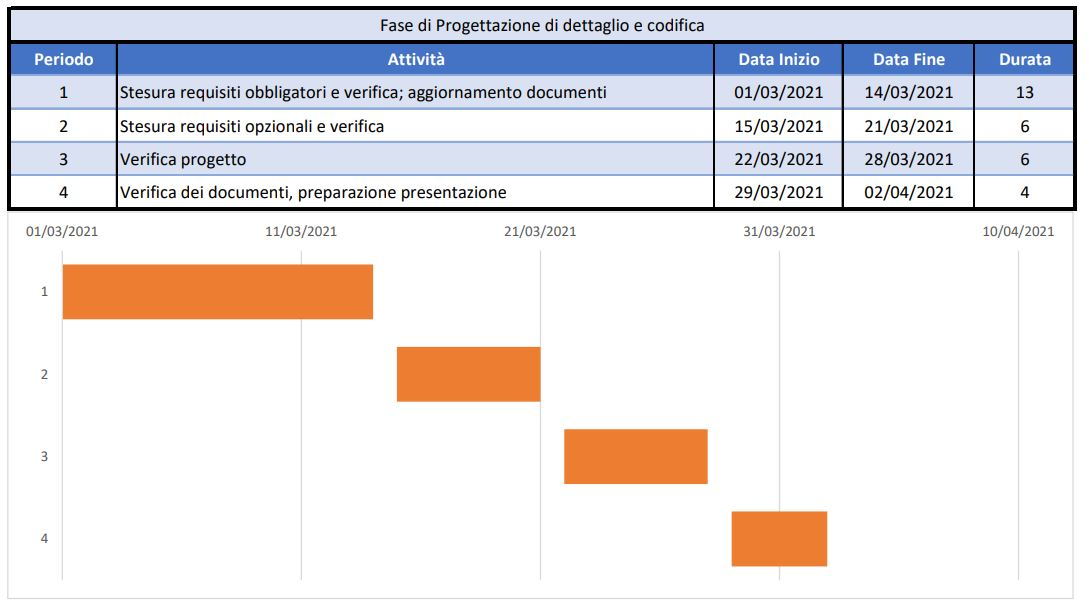
\includegraphics[width=12cm]{fase_dett_cod}
\caption{Diagramma di Gantt della fase di dettaglio e codifica}
\end{figure}


\subsection{Validazione e Collaudo}%
\label{sub:valid_coll}
Questa fase terminerà con la Revisione di Accettazione; in questo periodo verranno aggiornati i documenti e verrà verificato il software creato. 

\begin{figure}[H]
\centering
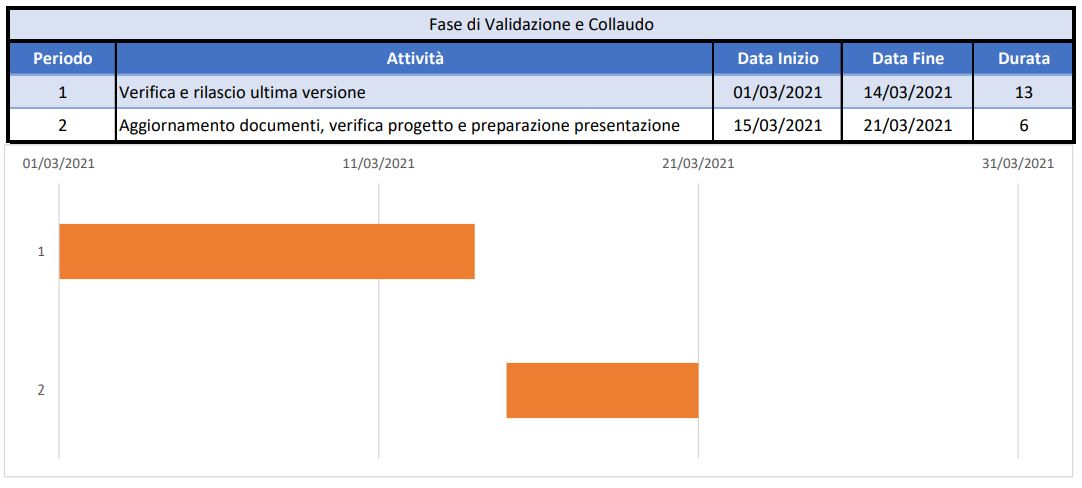
\includegraphics[width=12cm]{fase_valid_collaudo}
\caption{Diagramma di Gantt della fase di validazione e collaudo}
\end{figure}



\end{document}